\documentclass{beamer}

\usepackage{graphics}
\usepackage{graphicx}
\usepackage{amsmath,amssymb,amsthm}
\usepackage{color}
\usepackage{chemarr}
\usepackage{tikz}

%\usepackage{subeqnarray}
%\usepackage{easybmat}
%\usepackage{subfigure}

\newtheorem{prop}{Proposition}[section]
\newtheorem{defn}{Definition}[section]

%\usepackage{HA-prosper}
%\usepackage[dvips,letterpaper]{geometry}
\def\IC{\mathbb{C}}
\def\IF{\mathbb{F}}
\def\II{\mathbb{I}}
\def\IK{\mathbb{K}}
\def\IN{\mathbb{N}}
\def\IP{\mathbb{P}}
\def\IQ{\mathbb{Q}}
\def\IR{\mathbb{R}}
\def\IZ{\mathbb{Z}}

\def\C{\mathcal{C}}
\def\D{\mathcal{D}}
\def\I{\mathcal{I}}
\def\L{\mathcal{L}}
\def\M{\mathcal{M}}
\def\O{\mathcal{O}}
\def\Q{\mathcal{Q}}
\def\R{\mathcal{R}}
\def\U{\mathcal{U}}

\def\ba{\mathbf{a}}
\def\bb{\mathbf{b}}
\def\bc{\mathbf{c}}
\def\be{\mathbf{e}}
\def\bh{\mathbf{h}}
\def\bi{\mathbf{i}}
\def\bj{\mathbf{j}}
\def\bk{\mathbf{k}}
\def\bm{\mathbf{m}}
\def\bn{\mathbf{n}}
\def\bp{\mathbf{p}}
\def\br{\mathbf{r}}
\def\bs{\mathbf{s}}
\def\bu{\mathbf{u}}
\def\bv{\mathbf{v}}
\def\bw{\mathbf{w}}
\def\bx{\mathbf{x}}
\def\by{\mathbf{y}}
\def\bz{\mathbf{z}}

\def\bB{\mathbf{B}}
\def\bD{\mathbf{D}}
\def\bF{\mathbf{F}}
\def\bG{\mathbf{G}}
\def\bN{\mathbf{N}}
\def\bR{\mathbf{R}}
\def\bS{\mathbf{S}}
\def\bT{\mathbf{T}}
\def\b0{\mathbf{0}}



\def\R{\mathbb{R}}
%\def\Rzero{\mathcal{R}_0}
\def\diag{\textrm{diag}}
\def\tr{\textrm{tr}}
\def\det{\textrm{det}}
\def\sgn{\textrm{sgn}}
\def\imply{$\Rightarrow$}

\def\rank{\textrm{rank }}
\def\Sp{\textrm{Sp }}
\def\Span{\textrm{Span }}
\def\Tr{\textrm{Tr }}
\def\Mn{\mathcal{M}_n}
\def\NN#1{\|#1\|}
\def\N3#1{|\!|\!|#1|\!|\!|}
\def\diag{\textrm{diag}}
\def\tr{\textrm{tr}}
\def\ker{\textrm{Ker }}
\def\Proba#1{\P(#1)}
\def\Rzero{\mathcal{R}_0}

\usetheme{Boadilla}
%\usetheme{Singapore}

\AtBeginSection[]
{
\begin{frame}<beamer>
\frametitle{Outline}
\tableofcontents[currentsection]
\end{frame}
}

%%%%%%% 
%% Definitions in yellow boxes
\usepackage{etoolbox}
\newtheorem{importanttheorem}[theorem]{Theorem}
\newtheorem{importantproperty}[theorem]{Property}
\BeforeBeginEnvironment{importanttheorem}{%
	\setbeamercolor{block title}{fg=black,bg=red!50!white}
	\setbeamercolor{block body}{fg=black, bg=red!30!white}
}
\AfterEndEnvironment{importanttheorem}{
	\setbeamercolor{block title}{use=structure,fg=structure.fg,bg=structure.fg!20!bg}
	\setbeamercolor{block body}{parent=normal text,use=block title,bg=block title.bg!50!bg, fg=black}
}


%\AtBeginSubsection[]
%{
%\begin{frame}<beamer>
%\frametitle{Outline}
%\tableofcontents[currentsection,currentsubsection]
%\end{frame}
%}
%
%%\usepackage{HA-prosper}
%\usepackage[dvips,letterpaper]{geometry}

%\usetheme{Singapore}

%\usetheme{Pittsburgh}
%\usecolortheme{dove}
%\usecolortheme[rgb={0.3,0.3,0.3}]{structure}

\graphicspath{{./figures}}


\begin{document}
%\title{Mathematical biology}
%\author{St\'ephanie Portet}
%\institute[UofM]{University of Manitoba}

\title{Curve fitting}
\institute[Fall 2023]{MATH 3610}



\maketitle

%\frame{\frametitle{Outline}\tableofcontents }

\frame{\frametitle{Curve fitting}
\begin{itemize}
\item {\bf Data:} Limited number of data points representing values of a function for a limited number of values of the independent variable (e.g. time, space, $\dots$). 
\begin{itemize}
	\item $n$ data points $(x_i,y_i)$ with $i=1,\cdots, n$
\end{itemize}
\item {\bf Hypothesize the form of the function} \begin{itemize}
	\item $y=f(x,p)$ where $p$ is a $m-$vector of parameters ($m$ parameters)
\end{itemize}
\item 
%{\bf Interpolation:} estimate values of data for intermediate values of the independent variable 
%$\Rightarrow$ 
{\bf Curve fitting} (find the curve that has the best fit to data points) The best fit minimizes the difference between the actual value (data) and the predicted value (curve)
\begin{itemize}
	\item $\Rightarrow$ find the estimate of parameter values
\end{itemize}
\end{itemize}

}

\frame{\frametitle{Curve fitting: method of least-squares }
	{\bf Model}: $f(x,p)$ with parameters $p$\\
	{\bf Criterion}: measure the total error in fitting a curve to data
	$$RSS(p)=\sum_{i=1}^n(y_i-f(x_i,p))^2$$
		\begin{itemize}
			\item sum of squares for error = sum of squared residuals 
			\item residual = difference between the actual value (data) and the predicted value (curve)
		\end{itemize}
	{\bf Aim}: minimization of the sum of squared residual
$$\min_{p}RSS(p)$$
	{\bf Result}: Least-squares best fit minimizes the sum of squares of vertical distances between data points and fitting curve points.
}


\frame{\frametitle{Optimization problems}
	When an analytic expression of the function $\Phi(p)$ to optimize is known
	\vfill
	\begin{block}{Theorem}
		A smooth function $\Phi(p)$ attains an local minimum (resp. maximum) at $\hat{p}$ if
		\begin{itemize}
			\item the gradient $\frac{\partial \Phi(p)}{\partial p}$ vanishes at $\hat{p}$
			\item and the Hessian $H(p)$ with $(i,j)th$ element $\frac{\partial^2 \Phi(p)}{\partial p_i \partial p_j}$ is positive definite (resp. negative definite) at $\hat{p}$, or
			$$z^TH(p)z>0 \textrm{( resp. $<0$)} $$
			where $z$ is any real vector.
		\end{itemize}
	\end{block}
	
	\vfill
	
	(If $\Phi(p)$ is non-smooth, the local extrema are at the discontinuity of $\Phi(p)$ or where the gradient $\frac{\partial \Phi(p)}{\partial p}$ is discontinuous or vanishes)
}

%\frame{\frametitle{Mathematical concepts}
%	\begin{block}{Function of two or more variables}
%		The expression of $$z=f(x,y)$$ is a {\bf function of two variables} if a unique value of $z$ is obtained from each ordered pair of real numbers $(x,y)$.
%	\end{block}
%	
%	\begin{itemize}
%		\item $x$ and $y$ are the independent variables, 
%		\item and $z$ is the dependent variable.
%	\end{itemize}
%}
%\frame{\frametitle{Mathematical concepts}
%\begin{block}{Partial Derivatives}
%	Let $z=f(x,y)$ be a function of two independent variables. Let all indicated limits exist. Then the {\bf partial derivative} of $f(x,y)$ with respect to $x$ is
%	$$f_x(x,y)=\frac{\partial f}{\partial x}=\lim_{h\to 0}\frac{f(x+h,y)-f(x,y)}{h},$$
%	the {\bf partial derivative} of $f(x,y)$ with respect to $y$ is
%	$$f_y(x,y)=\frac{\partial f}{\partial y}=\lim_{h\to 0}\frac{f(x,y+h)-f(x,y)}{h}.$$
%\end{block}
%
%If the indicated limits do not exist, then the partial derivatives do not exist.
%}
%
%
%\frame{\frametitle{Mathematical concepts}
%	\begin{block}{Second-order partial derivatives}
%		For a function $z=f(x,y)$, if the indicated partial derivative exists, then
%		$$\frac{\partial}{\partial x}\left (\frac{\partial f}{\partial x} \right )=\frac{\partial ^2 f}{\partial x^2}=f_{xx}(x,y)$$
%		$$\frac{\partial}{\partial x}\left (\frac{\partial f}{\partial y} \right )=\frac{\partial ^2 f}{\partial x\partial y}=f_{yx}(x,y)$$
%		$$\frac{\partial}{\partial y}\left (\frac{\partial f}{\partial y} \right )=\frac{\partial ^2 f}{\partial y^2}=f_{yy}(x,y)$$
%		$$\frac{\partial}{\partial y}\left (\frac{\partial f}{\partial x} \right )=\frac{\partial ^2 f}{\partial y\partial x}=f_{xy}(x,y)$$
%	\end{block}
%}

\frame{\frametitle{Functions of two variables}
	\begin{block}{Second derivative test}
			To find the relative extrema of $\Phi(x,y)$
			\begin{itemize}
				\item Compute critical points $(x_0,y_0)$ such that
				$\frac{\partial \Phi}{\partial x}(x_0,y_0)=0$ and $\frac{\partial \Phi}{\partial y}(x_0,y_0)=0$
				\item At the critical point $(x_0,y_0)$:
				\begin{itemize}
					\item If $\frac{\partial ^2 \Phi}{\partial x^2}(x_0,y_0)<0$
					and
					$\frac{\partial ^2 \Phi}{\partial x^2}(x_0,y_0)\frac{\partial ^2 \Phi}{\partial y^2}(x_0,y_0)-\left (\frac{\partial ^2 \Phi}{\partial x \partial y}(x_0,y_0)\right)^2>0$ 
					then 
					$\Phi(x,y)$ has a relative maximum at $(x_0,y_0)$.
					\item If $\frac{\partial ^2 \Phi}{\partial x^2}(x_0,y_0)>0$ 
					and
					$\frac{\partial ^2 \Phi}{\partial x^2}(x_0,y_0)\frac{\partial ^2 \Phi}{\partial y^2}(x_0,y_0)-\left (\frac{\partial ^2 \Phi}{\partial x \partial y}(x_0,y_0)\right)^2>0$ 
					then
					$\Phi(x,y)$ has a relative minimum at $(x_0,y_0)$.
					\item If $\frac{\partial ^2 \Phi}{\partial x^2}(x_0,y_0)\frac{\partial ^2 \Phi}{\partial y^2}(x_0,y_0)-\left (\frac{\partial ^2 \Phi}{\partial x \partial y}(x_0,y_0)\right)^2<0$ 
					then there is a saddle point at $(x_0,y_0)$.
					\item If $\frac{\partial ^2 \Phi}{\partial x^2}(x_0,y_0)\frac{\partial ^2 \Phi}{\partial y^2}(x_0,y_0)-\left (\frac{\partial ^2 \Phi}{\partial x \partial y}(x_0,y_0)\right)^2=0$, no conclusive.
				\end{itemize} 
			\end{itemize}
	\end{block}

}

\frame{\frametitle{Method of least-squares for models linear in parameters}
	Aim: find parameter values for the model which best fits data
	\begin{itemize}
		\item {\bf Observation}: $n$ data points $(x_i,y_i)$ with $i=1,\cdots, n$ 
		\item {\bf Model}: $f(x,p)$ where $p$ is a $m-$vector of parameters ($m$ parameters)
		\item {\bf Criterion}: sum, $RSS$, of squared residuals 
		$$RSS(p)=\sum_{i=1}^n(y_i-f(x_i,p))^2$$
		\item {\bf Solution}: $\hat p$ such that
		$$RSS(\hat p)=\min_{p}RSS(p)$$
		is obtained by setting the gradient equal to zero ($m$ parameters)
		$$\frac{\partial RSS}{\partial p_j}=0,\quad j=1,\cdots , m$$
		or
		$$-2\sum_{i=1}^n(y_i-f(x_i,p))\frac{\partial f(x_i,p)}{\partial p_j}=0,\quad j=1,\cdots , m$$
		
	\end{itemize}
}


	\frame{\frametitle{US population (in millions) from 1790 to 2000}
	\vspace{-.1cm}
	\begin{minipage}{0.25\linewidth}
		\begin{center}
			{\footnotesize \begin{tabular}{c|c}
					1790 & 3.929\\
					1800 & 5.308\\
					1810 & 7.240\\
					1820 & 9.638\\
					& 12.866\\
					& 17.069\\ 
					& 23.192\\ 
					& 31.443\\
					& 38.558 \\
					& 50.156\\
					& 62.948\\
					1900 & 76.212\\
					& 92.228\\
					& 106.021\\
					& 123.202\\
					& 132.164\\
					& 151.325\\
					& 179.323\\
					& 203.302\\
					& 226.542\\
					& 248.709\\
					2000 & 281.421
			\end{tabular}}
		\end{center}
	\end{minipage}
	\begin{minipage}{0.7\linewidth}
		\begin{center}
			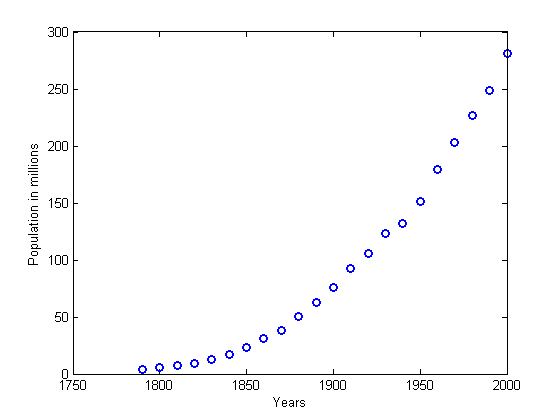
\includegraphics[scale=.6]{LS}\\
			{\bf Observation:} 22 data points $(x_i,y_i)=$ (year,population) with $i=1,\dots, 22$
		\end{center}
	\end{minipage}
}



	



\frame{\frametitle{US population (in millions) from 1790 to 2000}
	{\bf Model}: $f(x,p)$ where $p$ is a $k-$vector of parameters ($k$ parameters)
	\vfill
	Hypothesize the form of the function $f$
	\begin{itemize}
		\item {\bf Quadratic function} ($x$ years)
		$$f(x)=y=a+bx+cx^2$$
		$k=3$ parameters to estimate $a$, $b$ and $c$
		\item {\bf Exponential function} ($x$ years)
		$$f(x)=y=a \exp^{bx}$$
		Change of variable $\ln y =Y$
		$$\ln y = Y = \ln a + bx= A+ bx$$
		$k=2$ parameters to estimate $A$ and $b$
	\end{itemize}
	\alert{Both models are linear in parameters}
}	


\frame{\frametitle{Nonhomogeneous linear systems}
	To solve a nonhomogeneous linear systems ($\det (A)\not =0$)
	$$AX=B$$
	\begin{itemize}
		\item Find the inverse of the coefficient matrix and multiply the nonhomogeneous term by the inverse: $$X=A^{-1}B$$
		\item Cramer's rule
			\begin{theorem}[Cramer's rule]
			Consider the linear system $AX=B$ with $A\in\M_n$ a square matrix such that $|A|\neq 0$, $X=(x_1,\ldots,x_n)^T$ and $B=(b_1,\ldots,b_n)^T$ column vectors. Then for $i=1,\ldots,n$,
			\[
			x_i=\frac{|A_i|}{|A|},
			\]
			where $A_i$ is the matrix obtained by replacing column $i$ in $A$ by $B$.
		\end{theorem}
	\end{itemize}
}	


\frame{\frametitle{Method to find $A^{-1}$}
	\begin{theorem}[Direct method for inversion]
		Let $A$ be a $n\times n-$matrix. If $A$ is invertible ($|A|\not =0$), then elementary row operations on the augmented matrix $[A|I_n]$ eventually lead to the augmented matrix $[I_n|A^{-1}]$.
	\end{theorem}
	\begin{block}{Adjoint method}
		For $2\times 2-$matrix:	$
		A=\left[\begin{array}{cc}
			a & b \\
			c & d
		\end{array}\right], \quad A^{-1}=\frac{1}{ad-bc}\left[\begin{array}{cc}
			d & -b \\
			-c & a
		\end{array}\right]
		$
	\end{block}	

}



\frame{\frametitle{US population (in millions) from 1790 to 2000}
	
	Find the minimum of
	$$RSS(A,b)=\sum_{i=1}^n(\ln y_i-(A+bx_i))^2$$
	Set the gradient of $RSS$ to zero
	\begin{align*}
		\sum_{i=1}^n(\ln y_i-(A+bx_i))\frac{\partial (A+bx_i)}{\partial A}=&\sum_{i=1}^n(\ln y_i-(A+bx_i))=0\\\sum_{i=1}^n(\ln y_i-(A+bx_i))\frac{\partial (A+bx_i)}{\partial b}=&\sum_{i=1}^n(\ln y_i-(A+bx_i))x_i=0
	\end{align*}
	
	%		\begin{align*}
		%		\sum_{i=1}^n(\ln y_i-(A+bx_i))=&0\\\sum_{i=1}^n(\ln y_i-(A+bx_i))x_i=&0
		%		\end{align*}
	$\hat{A}$ and $\hat{b}$ (estimate of $A$ and $b$) satisfy
	$$\left[\begin{matrix}
		n & \sum_{i=1}^n x_i\\
		\sum_{i=1}^n x_i & \sum_{i=1}^n x_i^2
	\end{matrix}\right]
	\left[\begin{matrix}
		\hat{A}\\\hat{b}
	\end{matrix}\right]
	=\left[\begin{matrix}
		\sum_{i=1}^n \ln y_i\\
		\sum_{i=1}^n x_i\ln y_i
	\end{matrix}\right]
	$$
}	


\frame{\frametitle{US population (in millions) from 1790 to 2000}
	%\vspace{-.1cm}
	\begin{center}
		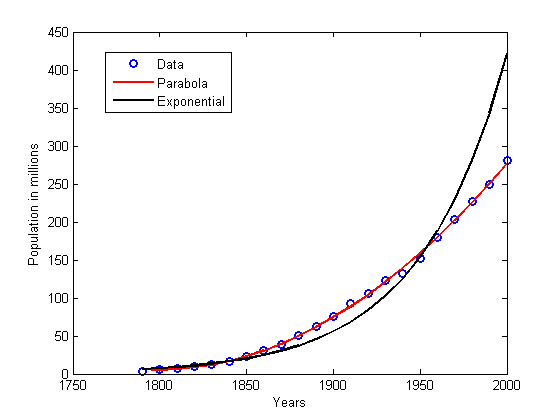
\includegraphics[scale=.75]{LS_all}
	\end{center}
%	Quadratic curve ($x$ years)
%	$$f(x)=0.0067x^2-24.0358x+21620.47$$
%	Exponential curve ($x$ years)
%	$$f(x)=1.2162\times 10^{-15}exp^{0.0202x}$$
}



\frame{\frametitle{Naive approach to compare models: $R^2$}
	Measure of the goodness of fit 
	\[R^2=1-\frac{RSS/n}{\sum(y_i-\bar{y})^2/n}\]
	where
	\begin{itemize}
		\item RSS = residual sum of squares
		\item $n$ = sample size
		\item $y$ = data
	\end{itemize}
	\vfill
	Select the model that maximizes $R^2$
	\vfill
	Best fit but neglect the model complexity (select the more parameter rich model)
	\vfill
	\alert{Only valid for linear models}
}

\frame{\frametitle{To compare models: Ajusted $R^2$}
	Replacing the two variances with their unbiased estimates 
	\vfill
	Measure of the goodness of fit 
	\[R_{adj}^2=1-\frac{RSS/(n-p-1)}{\sum(y_i-\bar{y})^2/(n-1)}\]
	where
	\begin{itemize}
		\item RSS = residual sum of squares
		\item $n$ = sample size
		\item $y$ = data
		\item $p$ = number of parameters
	\end{itemize}
	\vfill
	Select the model that maximizes $R_{adj}^2$
	\vfill
%	Best fit but neglect the model complexity (select the more parameter rich model)
%	\vfill
	\alert{Only valid for linear models}
}	
	
	
	\frame{\frametitle{Estimation of parameters in mechanistic models}
	$$\frac{dx}{dt}=m(x,p,t),\; x(t_0)=x_0(p),\; \tilde{y}=h(x,p,t)$$
	$x(t)$
	vector of state variables, $x_0$ IC, $h$ observable function and $p$ vector of unknown constant parameters
	\vfill
	To find the vector of parameter values $p$ that minimizes the distance between measured observations and simulated observations:
	\begin{itemize}
		\item Define a distance = Scalar objective function (cost function)
		$$F_{ls}(p)=\sum_{e=1}^{n_e}\sum_{o=1}^{n_o^e}\sum_{i=1}^{n_i^{e,o}}\omega_i^{e,o}(y_e^o(t_i)-\tilde{y}_o^e(t_i,p))^2$$
		
		$n_e$ $\#$ of experiments, $n_o^e$ $\#$ of observable per experiments, $n_i^{e,o}$ $\#$ of samples per observable per experiments
		
		$y_e^o(t_i)$ measured data, $\omega_i^{e,o}$ weights and $\tilde{y}_o^e(t_i,p)$ simulated output
		\item Optimization method to minimize $F_{ls}(p)$ to find $\hat{p}_{LSE}$ 
		$$F_{ls}(\hat{p}_{LSE})=\min_{p}F_{ls}(p)$$
	\end{itemize}
}	



\frame{\frametitle{Ordinary Differential Equations}
	\begin{defn}
		The following is an ordinary differential equation of the first order,
		\begin{equation}
			\frac{dx}{dt}=f(t,x), \tag{E}
		\end{equation}
		We also use the notation $x'=\frac{dx}{dt}$. 
	\end{defn}
	
	\begin{defn}
		Let $J=(a,b) = \{t\in \mathbb{R}: a<t<b\}$. A solution of the differential equation (E) on $J$ is a real-valued continuously differentiable function $\varphi$ defined on $J$ such that $(t,\varphi(t))\in D$ and
		\[\varphi'(t)=f(t,\varphi(t)),\]
		for all $t\in J$.
	\end{defn}
	($D$ an open connected subset of $\mathbb{R}^2$)
}	

\frame{\frametitle{Initial Value Problem}
	\begin{defn}
		Given $(\tau,\xi)\in D$, an {\bf initial value problem} (IVP) for (E) is given by 
		\begin{equation}
			x'=f(t,x), \quad x(\tau)=\xi
			\tag{I}
		\end{equation}
		where $x(\tau)=\xi$ is the initial condition.
	\end{defn}
	(A differential equation together with an initial condition form an Initial Value Problem (IVP))
	
	\begin{defn}
		A function $\varphi$ is a solution of (I) if $\varphi$ is a solution of the DE $x'=f(t,x)$ on some interval $J$ containing $\tau$ and also satisfies the initial condition $\varphi(\tau)=\xi$.
\end{defn}}






\frame{Different approaches to dealing with initial value problems:
	\begin{enumerate}
		\item Analytic methods - used to obtain the exact expression of solutions of a given equation
		\item Numerical methods - approximate, can be reasonably accurate. Yields approximations only locally on small intervals of the solution's domain
		\item Qualitative methods - to investigate properties of solutions without necessarily finding those solutions (existence, uniqueness, stability, or chaotic or asymptotic behaviors)
\end{enumerate}}	




\frame{ \frametitle{Separable equations} 
	\begin{block}{Definition}
		A first order DE
		$$\frac{dy}{dx}=f(x,y)$$
		
		is said to be separable or to have separable variables if it can be
		expressed as follows
		$$\frac{dy}{dx}=g(x)h(y).$$
	\end{block}
	(the vector field can be expressed as a product of a function of
	the independent variable times a function of the dependent variable
	)
	%\vspace{1cm} OR (from the textbook)
	%
	%If an equation can be written as
	%$$M(x)+N(y)\frac{dy}{dx}=0$$
	%the equation is said to be separable.
	%
	%
	%
	%($N(y)=\frac{1}{h(y)}$ and $M(x)=-g(x)$)
	
}


\frame{ \frametitle{Method to solve separable equations
		$\frac{dy}{dx}=g(x)h(y)$} {\tiny
		\begin{enumerate}
			\item Express the separable equation as follows
			$$\frac{1}{h(y(x))}\frac{dy}{dx}=g(x)$$
			\item As $y$, $\frac{dy}{dx}$, and $g(x)$ are functions of $x$,
			integrate with respect to $x$
			$$\int \frac{1}{h(y(x))}\frac{dy}{dx} dx=\int g(x) dx$$
			\item Use the Change of variable Theorem [if $u=v(x)$, $\int f(v(x))v'(x)dx=\int
			f(u)du$] for the left side with $u=y(x)$
			$$\int \frac{1}{h(u)}du=\int g(x) dx$$
			$$\int \frac{1}{h(y)}dy=\int g(x) dx$$
			\item Integrate
			\begin{equation}H(y)=G(x)+c\label{eq:GS}\end{equation} $c$ is the combination of the left
			and right integration constants, $H$ and $G$ are antiderivatives of
			$\frac{1}{h(y)}$ and $g(x)$ respectively.
			% \item Solve equation
			%(\ref{eq:GS}) for $y$ to obtain a explicit form of the general
			%solution.
	\end{enumerate}}
	
	
	
}



	\frame{\frametitle{Identifiability}
	Can unknown model parameters uniquely be determined by parameter estimation from
	measured data? $\Rightarrow$ Identifiability
	\vspace{1cm}
	
	
	Two problems: 
	\begin{enumerate} 
		\item the larger the number of
		unknown parameters in a model, the larger the amount of
		quantitative data necessary to determine meaningful values
		for these parameters (Practical identifiability)
		\item even if appropriate experimental
		data are available, model parameters may not be
		uniquely identifiable (Structural identifiability)
	\end{enumerate}
}


\frame{\frametitle{Identifiability}
	Profiles of error as a function of parameters to be estimated
	\begin{center}
		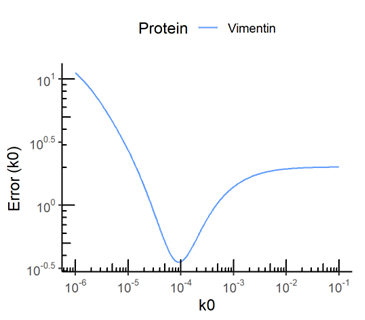
\includegraphics[scale=0.45]{figures/Error_Identifiable}
		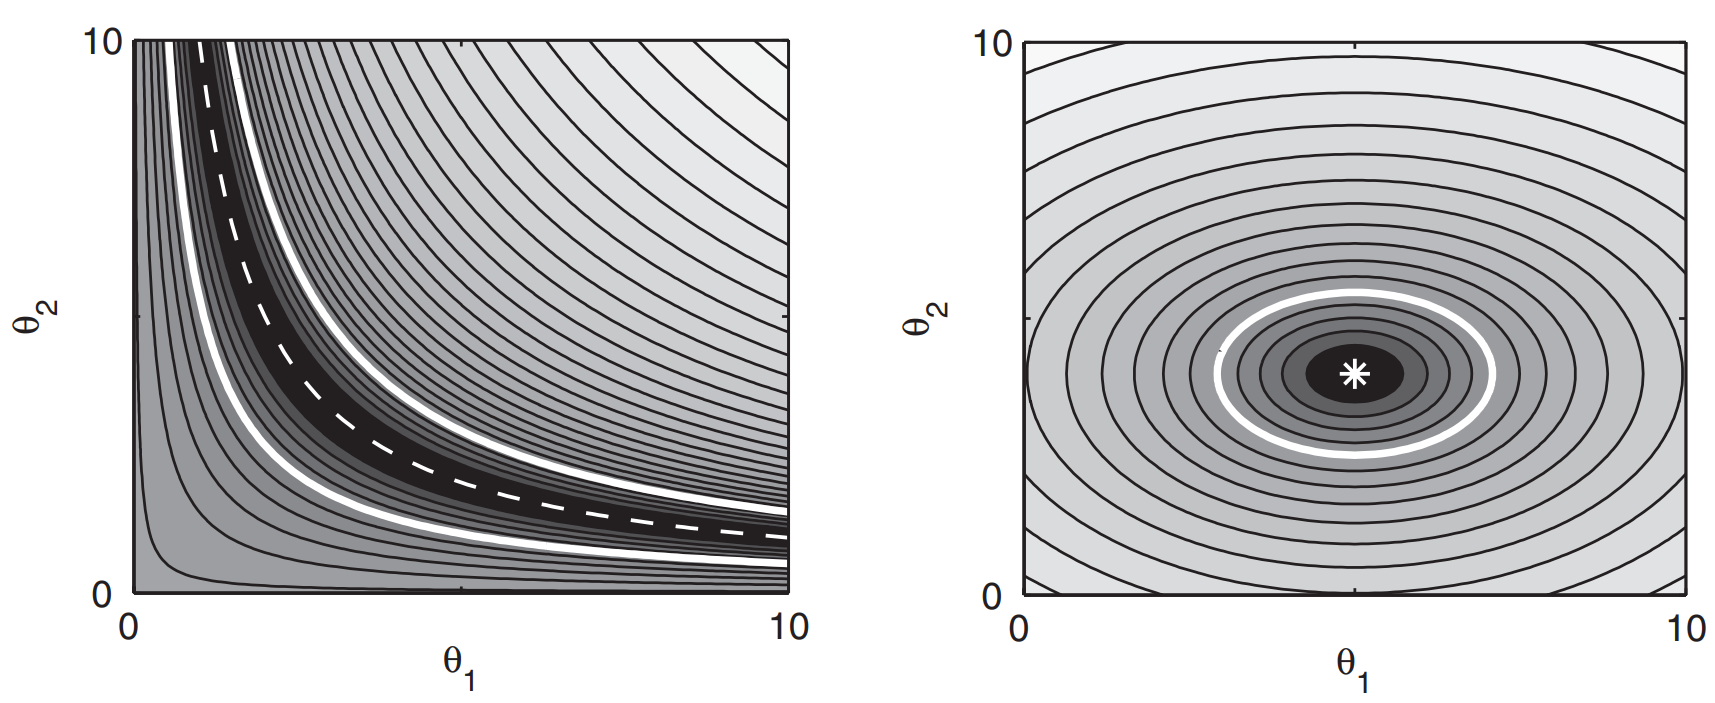
\includegraphics[scale=0.2]{figures/Error_Identifiable2d}
	\end{center}
}	



\frame{\frametitle{Optimization methods}
	When an analytic expression of the function to optimize is unknown
	\vfill
	\begin{itemize}
		\item Local optimization methods: 
		\begin{itemize}
			\item gradient descent-based methods: Levenberg-Marquardt or Gauss-Newton 
			\item derivative-free local search methods: Nelder-Mead method
			\item only find a global optimum for appropriate starting points
			\item converge to local optima 
			\item suboptimal solutions
		\end{itemize}
		\item Global optimization methods: %metaheuristic methods
		\begin{itemize}
			\item simulated annealing
			\item genetic algorithm
			\item particle swarm
		\end{itemize}
	\end{itemize}
	
	{\tiny Pitt and Banga (2019) BMC Bioinformatics. 20:82. Sagar {\it et al.} (2018) BMC Systems Biology 12:87. }
}

%%%%%%%%%%%%%%%%%%%%%%%%%%
%%%%%%%%%%%%%%%%%%%%%%%%%%
%%%%%%%%%%%%%%%%%%%%%%%%%%
%%%%%%%%%%%%%%%%%%%%%%%%%%
\section{Least squares, the other version..}

\begin{frame}{The least squares problem (simplest version)}
	\begin{definition}
		Given a collection of points $(x_1,y_1),\ldots,(x_n,y_n)$, find the coefficients $a,b$ of the line $y=a+bx$ such that
		$$
		\|\mathbf{e}\|=\sqrt{\varepsilon_1^2+\cdots+\varepsilon_n^2}
		=\sqrt{(y_1-\tilde y_1)^2+\cdots+(y_n-\tilde y_n)^2}
		$$
		is minimal, where $\tilde y_i=a+bx_i$ for $i=1,\ldots,n$
	\end{definition}
	\vfill
	We can solve this by brute force using, e.g., a genetic algorith to minimise $\|e\|$. Let us now see how to solve this problem ``properly''
\end{frame}


\begin{frame}
	For a data point $i=1,\ldots,n$
	\[
	\varepsilon_i = y_i-\tilde y_i = y_i - (a+bx_i)
	\]
	So if we write this for all data points,
	\begin{align*}
	\varepsilon_1 &= y_1 - (a+bx_1) \\
	&\;\;\vdots \\
	\varepsilon_n &= y_n - (a+bx_n) \\
	\end{align*}
	In matrix form
	\[
	\be = \bb-A\bx
	\]
	with
	\[
	\be = \begin{pmatrix}
	\varepsilon_1\\ \vdots\\ \varepsilon_n
	\end{pmatrix},
	A=\begin{pmatrix}
	1 & x_1 \\ \vdots & \vdots \\ 1 & x_n
	\end{pmatrix},
	\bx = \begin{pmatrix}
	a\\b
	\end{pmatrix}\textrm{ and }
	\bb = \begin{pmatrix}
	y_1\\ \vdots\\ y_n
	\end{pmatrix}
	\]
\end{frame}

\begin{frame}{The least squares problem (reformulated)}
\begin{definition}[Least squares solutions]
Consider a collection of points $(x_1,y_1),\ldots,(x_n,y_n)$, a matrix $A\in\M_{mn}$, $\bb\in\IR^m$. A \textbf{least squares solution} of $A\bx=\bb$ is a vector $\tilde \bx\in\IR^n$ s.t.
\[
\forall \bx\in\IR^n,\quad \|\bb-A\tilde\bx\|\leq \|\bb-A\bx\|
\]
\end{definition}
\end{frame}


\begin{frame}{Needed to solve the problem}
\begin{definition}[Best approximation]
Let $V$ be a vector space, $W\subset V$ and $\mathbf{v}\in V$. The \textbf{best approximation} to $\mathbf{v}$ in $W$ is $\tilde{\mathbf{v}}\in W$ s.t.
\[
\forall\mathbf{w}\in W, \mathbf{w}\neq\tilde{\mathbf{v}}, \quad
\|\mathbf{v}-\tilde{\mathbf{v}}\| < \|\mathbf{v}-\mathbf{w}\|
\]
\end{definition}
\vfill
\begin{theorem}[Best approximation theorem]
Let $V$ be a vector space with an inner product, $W\subset V$ and $\mathbf{v}\in V$. Then $\mathsf{proj}_W(\mathbf{v})$ is the best approximation to $\mathbf{v}$ in W
\end{theorem}
\end{frame}


\begin{frame}{Let us find the least squares solution}
$\forall \bx\IR^n$, $A\bx$ is a vector in the \textbf{column space} of $A$ (the space spanned by the vectors making up the columns of $A$)
\vfill
Since $\bx\in\IR^n$, $A\bx\in\mathsf{col}(A)$
\vfill
$\implies$ least squares solution of $A\bx=\bb$ is a vector $\tilde\by\in\mathsf{col}(A)$ s.t.
\[
\forall\by\in\mathsf{col}(A),\quad\|\bb-\tilde\by\|\leq\|\bb-\by\|
\]
\vfill
This looks very much like Best approximation and Best approximation theorem
\end{frame}

\begin{frame}{Putting things together}
We just stated: The least squares solution of $A\bx=\bb$ is a vector $\tilde\by\in\mathsf{col}(A)$ s.t.
\[
\forall\by\in\mathsf{col}(A),\quad\|\bb-\tilde\by\|\leq\|\bb-\by\|
\]
\vfill
We know (reformulating a tad):
\begin{theorem}[Best approximation theorem]
Let $V$ be a vector space with an inner product, $W\subset V$ and $\mathbf{v}\in V$. Then $\mathsf{proj}_W(\mathbf{v})\in W$ is the best approximation to $\mathbf{v}$ in W, i.e.,
\[
\forall\mathbf{w}\in W, \mathbf{w}\neq\mathsf{proj}_W(\mathbf{v}), \quad
\|\mathbf{v}-\mathsf{proj}_W(\mathbf{v})\| < \|\mathbf{v}-\mathbf{w}\|
\]
\end{theorem}
\vfill
$\implies$ $W=\mathsf{col}(A)$, $\bv=\bb$ and $\tilde\by=\mathsf{proj}_{\mathsf{col}(A)}(\mathbf{b})$
\end{frame}

\begin{frame}
So if $\tilde\bx$ is a least squares solution of $A\bx=\bb$, then
\[
\tilde\by = A\tilde\bx = \mathsf{proj}_{\mathsf{col}(A)}(\mathbf{b})
\]
\vfill
We have
\[
\bb-A\tilde\bx = \bb-\mathsf{proj}_{\mathsf{col}(A)}(\mathbf{b}) 
= \mathsf{perp}_{\mathsf{col}(A)}(\mathbf{b})
\]
and it is easy to show that
\[
\mathsf{perp}_{\mathsf{col}(A)}(\mathbf{b}) \perp \mathsf{col}(A)
\]
\vfill
So for all columns $\ba_i$ of $A$
\[
\ba_i\boldsymbol{\cdot}(\bb-A\tilde\bx) = 0
\]
which we can also write as $\ba_i^T(\bb-A\tilde\bx) = 0$
\end{frame}

\begin{frame}
For all columns $\ba_i$ of $A$,
\[\ba_i^T(\bb-A\tilde\bx) = 0
\]
\vfill
This is equivalent to saying that
\[
A^T(\bb-A\tilde\bx) = \b0
\]
\vfill
We have
\begin{align*}
A^T(\bb-A\tilde\bx) = \b0 &\iff A^T\bb - A^TA\tilde\bx = \b0 \\
&\iff A^T\bb = A^TA\tilde\bx \\
&\iff A^TA\tilde\bx = A^T\bb
\end{align*}
The latter system constitutes the \textbf{normal equations} for $\tilde\bx$
\end{frame}


\begin{frame}{Least squares theorem}
\begin{importanttheorem}[Least squares theorem]\label{th:least_squares}
$A\in\M_{mn}$, $\bb\in\IR^m$. Then
\begin{enumerate}
\item $A\bx=\bb$ always has at least one least squares solution $\tilde\bx$
\item $\tilde\bx$ least squares solution to $A\bx=\bb$ $\iff$ $\tilde\bx$ is a solution to the normal equations $A^TA\tilde\bx = A^T\bb$
\item $A$ has linearly independent columns $\iff$ $A^TA$ invertible.  
\newline In this case, the least squares solution is unique and 
\[
\tilde\bx = \left(A^TA\right)^{-1}A^T\bb
\]
\end{enumerate}
\end{importanttheorem}
\vfill
We have seen 1 and 2, we will not show 3 (it is not hard)
\end{frame}


\begin{frame}{Suppose we want to fit something a bit more complicated..}
For instance, instead of the affine function
\[
y = a+bx
\]
suppose we want to do the quadratic
\[
y = a_0+a_1x+a_2x^2
\]
or even
\[
y = k_0 e^{k_1x}
\]
\vfill
How do we proceed?
\end{frame}


\begin{frame}{Fitting the quadratic}
We have the data points $(x_1,y_1),(x_2,y_2),\ldots,(x_n,y_n)$ and want to fit
\[
y = a_0+a_1x+a_2x^2
\]
At $(x_1,y_1)$,
\[
\tilde y_1 = a_0+a_1x_1+a_2x_1^2
\]
$\vdots$\\
At $(x_n,y_n)$,
\[
\tilde y_n = a_0+a_1x_n+a_2x_n^2
\]
\end{frame}

\begin{frame}
In terms of the error
\begin{align*}
\varepsilon_1 &= y_1-\tilde y_1 = y_1-(a_0+a_1x_1+a_2x_1^2) \\
&\;\;\vdots\\
\varepsilon_n &= y_n-\tilde y_n = y_n-(a_0+a_1x_n+a_2x_n^2)
\end{align*}
i.e.,
\[
\be = \bb-A\bx 
\]
where
\[
\be = \begin{pmatrix}
\varepsilon_1\\ \vdots\\ \varepsilon_n
\end{pmatrix},
A=\begin{pmatrix}
1 & x_1 & x_1^2\\ \vdots & \vdots & \vdots \\ 1 & x_n & x_n^2
\end{pmatrix},
\bx = \begin{pmatrix}
a_0\\a_1\\a_2
\end{pmatrix}\textrm{ and }
\bb = \begin{pmatrix}
y_1\\ \vdots\\ y_n
\end{pmatrix}
\]
\vfill
Theorem~\ref{th:least_squares} applies, with here $A\in\M_{n3}$ and $\bb\in\IR^n$
\end{frame}


\begin{frame}{Fitting the exponential}
Things are a bit more complicated here
\vfill
If we proceed as before, we get the system
\begin{align*}
y_1 &= k_0 e^{k_1x_1} \\
&\;\;\vdots \\
y_n &= k_0 e^{k_1x_n}
\end{align*}
$e^{k_1x_i}$ is a nonlinear term, it cannot be put in a matrix
\vfill
\emph{However}: take the $\ln$ of both sides of the equation
\[
\ln(y_i) = \ln(k_0e^{k_1x_i}) = \ln(k_0)+\ln(e^{k_1x_i}) = \ln(k_0)+k_1x_i
\]
If $y_i,k_0>0$, then their $\ln$ are defined and we're in business..
\end{frame}

\begin{frame}
\[
\ln(y_i) = \ln (k_0)+k_1x_i
\]
So the system is
\begin{align*}
\by = A\bx+\bb
\end{align*}
with
\[
A = \begin{pmatrix}
x_1\\ \vdots \\ x_n
\end{pmatrix},
\bx = \begin{pmatrix}
k_1
\end{pmatrix},
\bb = \begin{pmatrix}
\ln (k_0)
\end{pmatrix}
\textrm{ and }
\by = \begin{pmatrix}
\ln (y_1)\\ \vdots\\ \ln (y_n)
\end{pmatrix}
\]
\end{frame}


\end{document}


